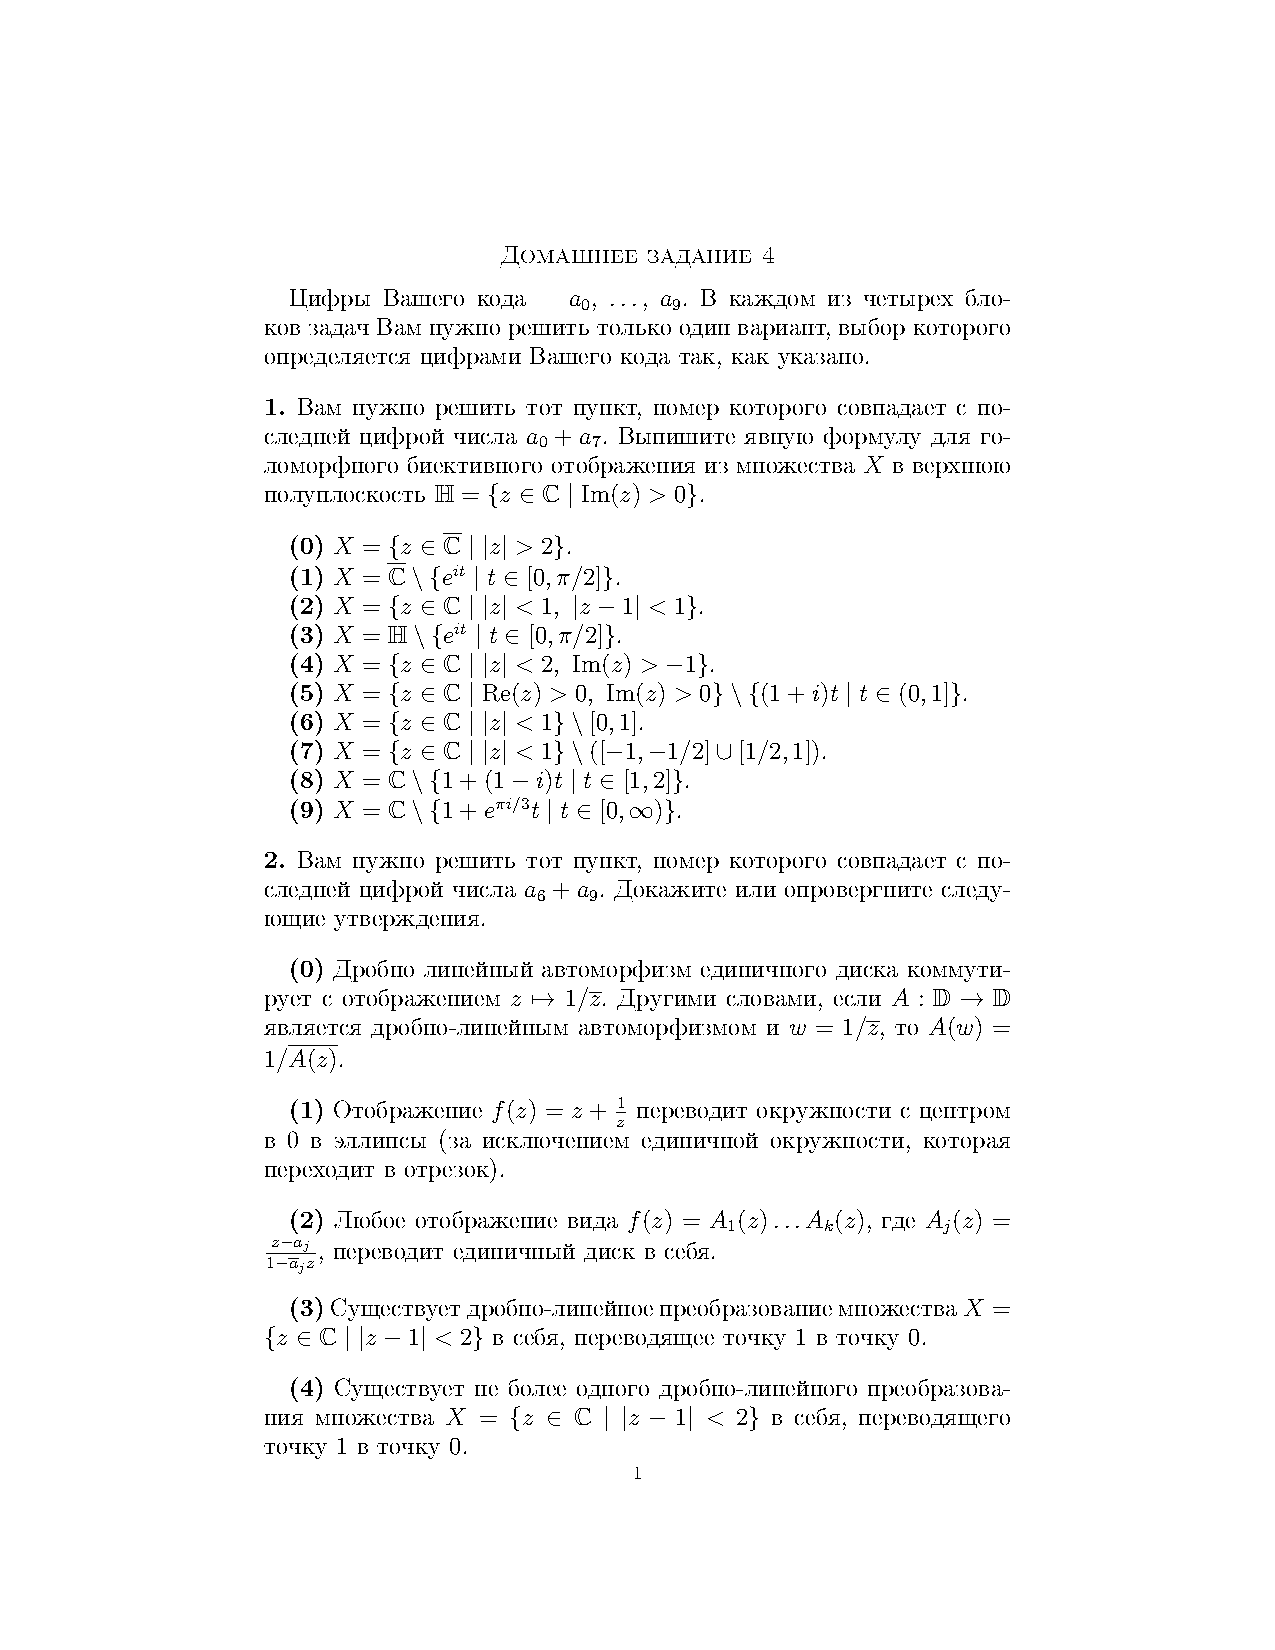
\includepdf[scale=1,pages=1-4]{Tasks/hw4}
\newpage
\section*{Решения}
\subsection*{Задача 1}
	Необходимо решить задачу $a_0 + a_7 = 1 + 3 = 4 \mod 10$
	\begin{gather*}
		X = \{z \in \mathbb{C}|\ |z| < 2,\ \Im(z) > -1\}\qquad
		\mathbb{H} = \{z \in \mathbb{C}|\ \Im(z) > 0\}
	\end{gather*}
	Заметим, что у $X$ есть 2 угла $\frac{2\pi}{3}$, тогда переведем один из них (пусть это будет точка $\sqrt{3}-i$) на бесконечность, а второй ($-\sqrt{3}-i$) в 0. И тогда, чтобы угол $\frac{2\pi}{3}$ стал равным $\pi$, необходимо возвести итоговое отображение в степень $\frac{3}{2}$.
	\begin{gather*}
		f(z) = \frac{az + b}{cz + d}\\
		\begin{cases}
			f(\sqrt{3}-i) = \frac{a(\sqrt{3}-i) + b}{c(\sqrt{3}-i) + d} = \infty\qquad
			c(\sqrt{3}-i) + d = 0\\
			f(-\sqrt{3}-i) = \frac{a(-\sqrt{3}-i) + b}{c(-\sqrt{3}-i) + d} = 0\qquad
			a(-\sqrt{3}-i) + b = 0
		\end{cases}\\
		f(z) = \frac{az + (\sqrt{3}+i)a}{cz + (i - \sqrt{3})c}
		= \frac{a}{c}\cdot\frac{z + i + \sqrt{3}}{z + i - \sqrt{3}}\\
		f_1(z) = f(z)^{\frac{3}{2}}
		= \left(\frac{a}{c}\cdot\frac{z + i + \sqrt{3}}{z + i - \sqrt{3}}\right)^{\frac{3}{2}}
	\end{gather*}
	Осталось заметить, что данное преобразование дает нам полуплоскость $\{\Re(z) < 0\}$, это можно проверить, посмотрев куда переходит центр окружности $\frac{0 + i + \sqrt{3}}{0 + i - \sqrt{3}}^{\frac{3}{2}} = -1$, тогда для получения отображения необходимо повернуть все на $\frac{\pi}{2}$ против часовой стрелки, то есть домножить на $-i$, откуда
	\begin{gather*}
		F(z) = -i \cdot \left(\frac{a}{c}\cdot\frac{z + i + \sqrt{3}}{z + i - \sqrt{3}}\right)^{\frac{3}{2}},\quad \frac{a}{c} \in \mathbb{R}
	\end{gather*}
\vskip 0.4in

\subsection*{Задача 2}
	Необходимо решить задачу $a_6 + a_9 = 9 + 6 = 5 \mod 10$\\
	Мы можем задать окружность 3 точками, поэтому будем рассматривать автоморфизм $(x_1, x_2, x_3) \mapsto (y_1, y_2, y_3)$, обозначим его как $\Phi$ и $\Phi(x_i) = y_i$. Заметим, что $\operatorname{PSL}(2, \mathbb{R})$ -- автоморфизмы верхней полуплоскости и
	\begin{gather*}
		z \to \frac{az + b}{cz + d}\\
		ad - bc = 1\\
		(a,b,c,d) \sim (\alpha a, \alpha b,\alpha c,\alpha d)
	\end{gather*}
	То есть эти матрицы задаются 3 параметрами (так как 4 получается из $ad - bc = 1$). Тогда заметим, что у нас есть система из 4 уравнений с 4 неизвестными:
	\begin{gather*}
		\frac{ax_1 + b}{cx_1 + d} = y_1\qquad
		\frac{ax_2 + b}{cx_2 + d} = y_2\qquad
		\frac{ax_3 + b}{cx_3 + d} = y_3\qquad
		ad-bc = 1
	\end{gather*}
	У это системы есть хотя бы одно решение, а следовательно есть и автоморфизм, переводящий одну окружность в другую.
	\begin{comment}
	Заметим, что можно построить биекцию из любого круга в любую полуплоскость, для определенности, $\mathbb{H} = \{\Im(z) > 0\}$, тогда если есть 2 круга $O_1, O_2$, то можно построить две биекции $f_1: O_1 \to \mathbb{H},\ f_2: \mathbb{H} \to O_2$ и $f_1 \circ f_2$ будет биекцией $O_1 \to O_2$, при это граница биективно отобразилась в границу, что и требовалось. 
	\end{comment}
\vskip 0.4in

\subsection*{Задача 3}
	Необходимо решить задачу $a_3 + a_9 = 9 + 6 = 5 \mod 10$
	\begin{gather*}
		U = \{x > y > 0\},\ (a,b) = (2, 1)
	\end{gather*}
	Переведем нашу область в полуплоскость, получим отображение
	$f_1(z) = z^4$ и $(2,1)$ перейдет в $(-7, 24)$.\\
	Теперь переведем полуплоскость $\mathbb{H}$ в окружность, но сперва переведем $(-7,24)$ в $(0,1)$
	\begin{gather*}
		f_2(z) = \frac{z+7}{24}\\
		f_3(z) = \frac{z-i}{z+i}\\
		f(z) = f_1 \circ f_2 \circ f_3
		= \frac{\frac{z^4+7}{24} - i}{\frac{z^4+7}{24} + i}
		= \frac{z^4 + 7 - 24i}{z^4 + 7 - 24i} 
	\end{gather*}
	Возьмем логарифм от $f(z)$, он перведет центр окружности в бексонечность, а края в 0, что и трбовалось
	\begin{gather*}
		F(z) = \log(f(z))
		= \log\left( \frac{z^4 + 7 - 24i}{z^4 + 7 - 24i} \right)
	\end{gather*}

\vskip 0.4in
\subsection*{Задача 4}
	Необходимо решить задачу $3a_7 = 3 \cdot 3 = 9 \mod 10$
	\begin{gather*}
		X = \{z = x + iy|\ 0<x<\frac{\pi}{2}\},\quad f(z) = \sin(z)\\
		\sin(z)
		= \sin(x + iy)
		= \sin(x)\cos(iy) + i\cos(x)\sin(iy)
		= \sin(x)\cosh(y) + i\cos(x)\sinh(y)\\
		\Re(\sin(z)) = \sin(x)\cosh(y),\quad \Im(\sin(z)) = \cos(x)\sinh(y)
	\end{gather*}
	Заметим что есть период $2\pi$, а следовательно достаточно рассмотреть $x \in (-\pi, \pi)$. Заметим, что
	\begin{gather*}
		u \left(\frac{\pi}{2} - x, y \right) = u\left( \frac{\pi}{2}+x, -y \right)\\
		v \left(\frac{\pi}{2}-x, y \right) = v \left( \frac{\pi}{2}+x, -y\right)
	\end{gather*}
	Тогда
	\begin{figure}[h]
	\begin{minipage}[h]{0.5\linewidth}
		
\includegraphics[width=0.95\linewidth]{Pic3}
		\caption{Комплексная плоскость}
	\end{minipage}
	\hfill
	\begin{minipage}[h]{0.5\linewidth}
		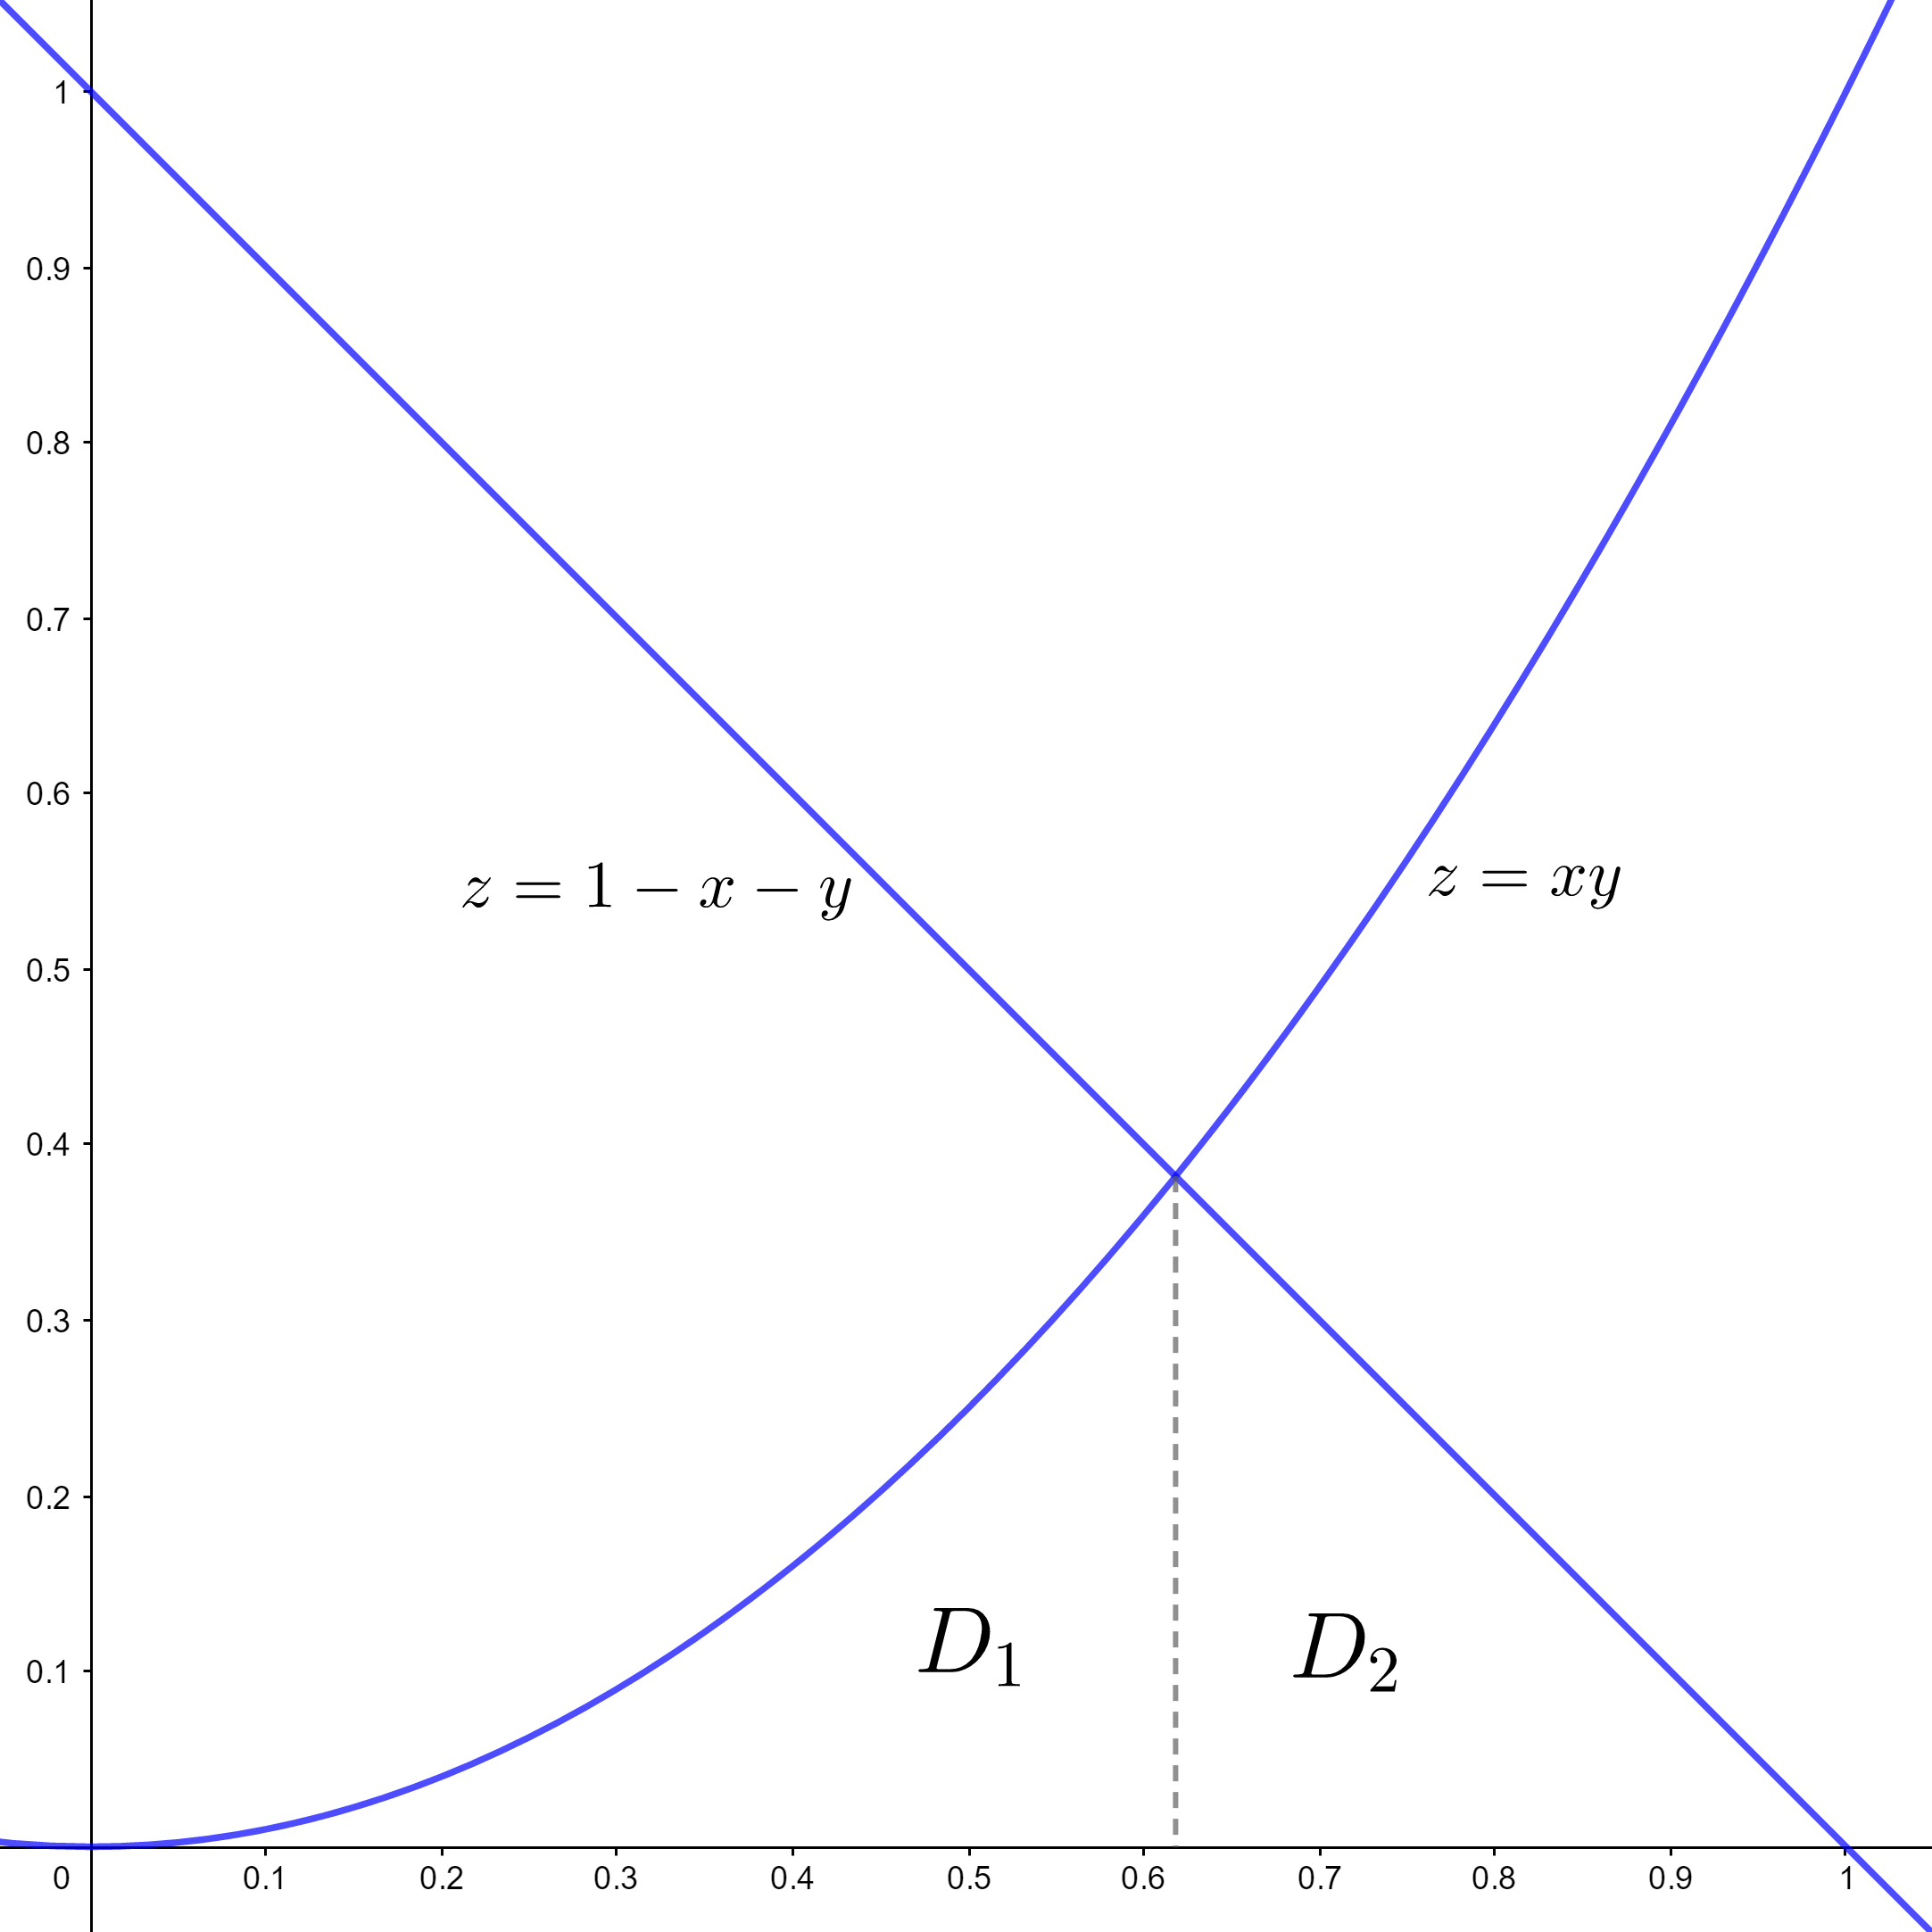
\includegraphics[width=0.95\linewidth]{Pic4}
		\caption{Плоскость после преобразования $\sin z$ на $X$}
	\end{minipage}
	\end{figure}
\vskip 0.4in

\begin{comment}
\subsection*{Задача 5}
	Необходимо решить задачу $a_1 + a_8 = 7 + 8 = 5 \mod 10$
\end{comment}